\subsection{Case study}\label{subsec:case-study}
This section describes the practical experiment used to evaluate representations.
The goal was to validate the previous evaluation in a more realistic development scenario.
Additionally, this was an opportunity to assess the development experience that the notations deliver.

\subsubsection{Scenario and context}
The goal of this experiment was to evaluate the expressiveness of representations in a practical context.
This was achieved by recreating a few screens of a fictional application.
The application designed for this experiment was modeled after Trello\furl{trello.com} \textendash\ a well-known Web application for creating Kanban-style lists.
The choice was motivated by the application's popularity and relative complexity.

Capabilities of the original application are very broad and include detailed management of workspaces, users, boards, as well as editing and managing content-rich cards.
It would not be reasonable to implement all these functionalities \textendash\ to keep the experiment manageable, it was necessary to limit its scope.
The selected area to implement concerns simple management of cards across two views and a single dialog window:
\begin{itemize}
    \item the first view allows for viewing all boards the user has access to and navigating to a board
    \item the second view allows for viewing a particular board and its data \textendash\ name, columns and cards
    \item the dialog window allows for adding or editing a single card
\end{itemize}
This setup covers all four CRUD operations, making the experiment representative of real-life applications.
Management of boards and columns within a board was omitted to keep the example as small as possible.

Additionally, the representations should be able to represent two major components:
\begin{itemize}
    \item a card \textendash\ contains information about a title of a task, its description, assigned person and due date; it is also assigned to a column
    \item a column \textendash\ a board consists of multiple columns, each possibly containing multiple cards; additionally, to give it meaning, it also has a title
\end{itemize}

To further simplify the experiment, the interface was only implemented in a mobile version \textendash\ it is considered a good practice to design applications and website using the \enquote{mobile first} principle\furl{https://developer.mozilla.org/en-US/docs/Web/Progressive_web_apps/Responsive/Mobile_first}.

The subsequent paragraphs provide a descriptions of functionalities that the representations were expected to implement;
table~\ref{tab:case-study-requirements} summarizes them, split across five sections \textendash\ each corresponding to an implementation area described beforehand.
In this experiment, the requirements were not prescriptive \textendash\ they only listed \enquote{features} to implement, without specifying how should they be implemented.
This is meant to produce a more practical evaluation.
To reflect this freedom of implementation, the evaluation of requirements included a score for partial fulfillment, not only a binary score.

Each requirement RX.Y is assigned a score $R_{X.Y}$ based on formula~\ref{eq:3-4-requirement-scoring}
\begin{equation}
    R_{X.Y} =
    \begin{dcases}
        0,  & \text{if the requirement is not satisfied}\\
        0.5 & \text{if the requirement is partially satisfied}\\
        1   & \text{if the requirement is satisfied}
    \end{dcases}
    \label{eq:3-4-requirement-scoring}
\end{equation}

The score $R_X$ for each area RX is the average score of all the requirements for the area (formula~\ref{eq:3-4-area-scoring}):
\begin{equation}
    R_X = \frac{\sum_{i=1}^{n} R_{X.i}}{n}
    \label{eq:3-4-area-scoring}
\end{equation}

Similarly, the total score $T_{\text{requirements}}$ for the whole representation is\textellipsis.
\begin{equation}
    T_{\text{requirements}} = \frac{\sum_{i=1}^{5} R_i}{5}
    \label{eq:3-4-representation-scoring}
\end{equation}

\begin{longtblr}[
    caption = {Requirements for parts of the interface developed in the case study},
    label = {tab:case-study-requirements},
]{
    colspec = {cc},
    rowhead = 1,
    rows = {m},
}
    \hline[1pt]
    \textbf{Number} & \textbf{Requirement name}                                                       \\*
    \hline[1pt]
    \textbf{R1}     & \textbf{Boards view}                                                            \\*
    R1.1            & view title has a bold, very large font                                          \\*
    R1.2            & boards are loaded when the view is opened                                       \\*
    R1.3            & bords are displayed                                                             \\*
    R1.4            & clicking on a board navigates to the selected board                             \\
    \hline
    \textbf{R2}     & \textbf{Board view}                                                             \\*
    R2.1            & columns (and cards) are loaded when the view is opened                          \\*
    R2.2            & columns are displayed in a horizontal layout                                    \\*
    R2.3            & columns can be scrolled when they don't fit on the screen                       \\
    \hline
    \textbf{R3}     & \textbf{Column component}                                                       \\*
    R3.1            & container has some padding                                                      \\*
    R3.2            & title is displayed at the top (and doesn't move when scrolling cards)           \\*
    R3.3            & cards displayed in a column, slightly separated from one another                \\*
    R3.4            & cards can be scrolled when they don't fit                                       \\*
    R3.5            & new card button is displayed at the bottom (and doesn't move when scrolling)    \\*
    R3.6            & new card button is slightly separated from the cards and is centered            \\*
    R3.7            & new card button has a plus icon                                                 \\*
    R3.8            & new card button opens a card dialog without data when clicked                   \\
    \hline
    \textbf{R4}     & \textbf{Card component}                                                         \\*
    R4.1            & card button is displayed in the top right corner of the card                    \\*
    R4.2            & card button opens a context menu when clicked                                   \\*
    R4.3            & editing card item opens a dialog with card data when clicked                    \\*
    R4.4            & delete card item deletes the card from the column when clicked                  \\*
    R4.5            & delete card item calls an appropriate service when clicked                      \\*
    R4.6            & card indicators are written in grey text                                        \\*
    R4.7            & card indicators display icons                                                   \\
    \hline
    \textbf{R5}     & \textbf{Card dialog}                                                            \\*
    R5.1            & empty inputs have placeholders                                                  \\*
    R5.2            & title field is required                                                         \\*
    R5.3            & title field displays a custom error message when the input is empty             \\*
    R5.4            & card description field is a multi-row input                                     \\*
    R5.5            & assigned person and planned date fields are shorter and displayed in single row \\*
    R5.6            & planned date field is a date input                                              \\*
    R5.7            & column field allows selecting from all columns in the board                     \\*
    R5.8            & cancel button discards the changes                                              \\*
    R5.9            & save button adds or updates the card                                            \\*
    R5.10           & save button calls a service                                                     \\*
    R5.11           & save button is not active if the title is not provided                          \\
    \hline[1pt]
\end{longtblr}

\paragraph{The boards view}

\begin{figure}
    \centering
    
\includegraphics[height=0.4\textheight]{./3-research-methodology/boards-view}
    \caption{An example design of a boards view.}
    \label{fig:3-4-boards-view}
\end{figure}

The boards view (presented in figure~\ref{fig:3-4-boards-view}) is meant to be the entrypoint of the application.
In this case study, it is rather simple \textendash\ it only consists of the header and the list of boards of the user has access to.
The user can navigate to each of the boards by clicking a card with the board's name.
\todo{write clearer}Although in a real application, this view would provide much more functionality and information, as explained in the introduction to this section, this experiment only evaluates a narrow subset for brevity.

\todo[inline]{requirements}

\paragraph{The board view}
The board view, presented in figures~\ref{fig:3-4-board-view} and~\ref{fig:3-4-board-view-with-dialog} consists of a title and multiple columns.
Only the part with the green background is visible to the user;
the rest of the columns need to be scrolled to the view to be visible.

\begin{figure}
    \centering
    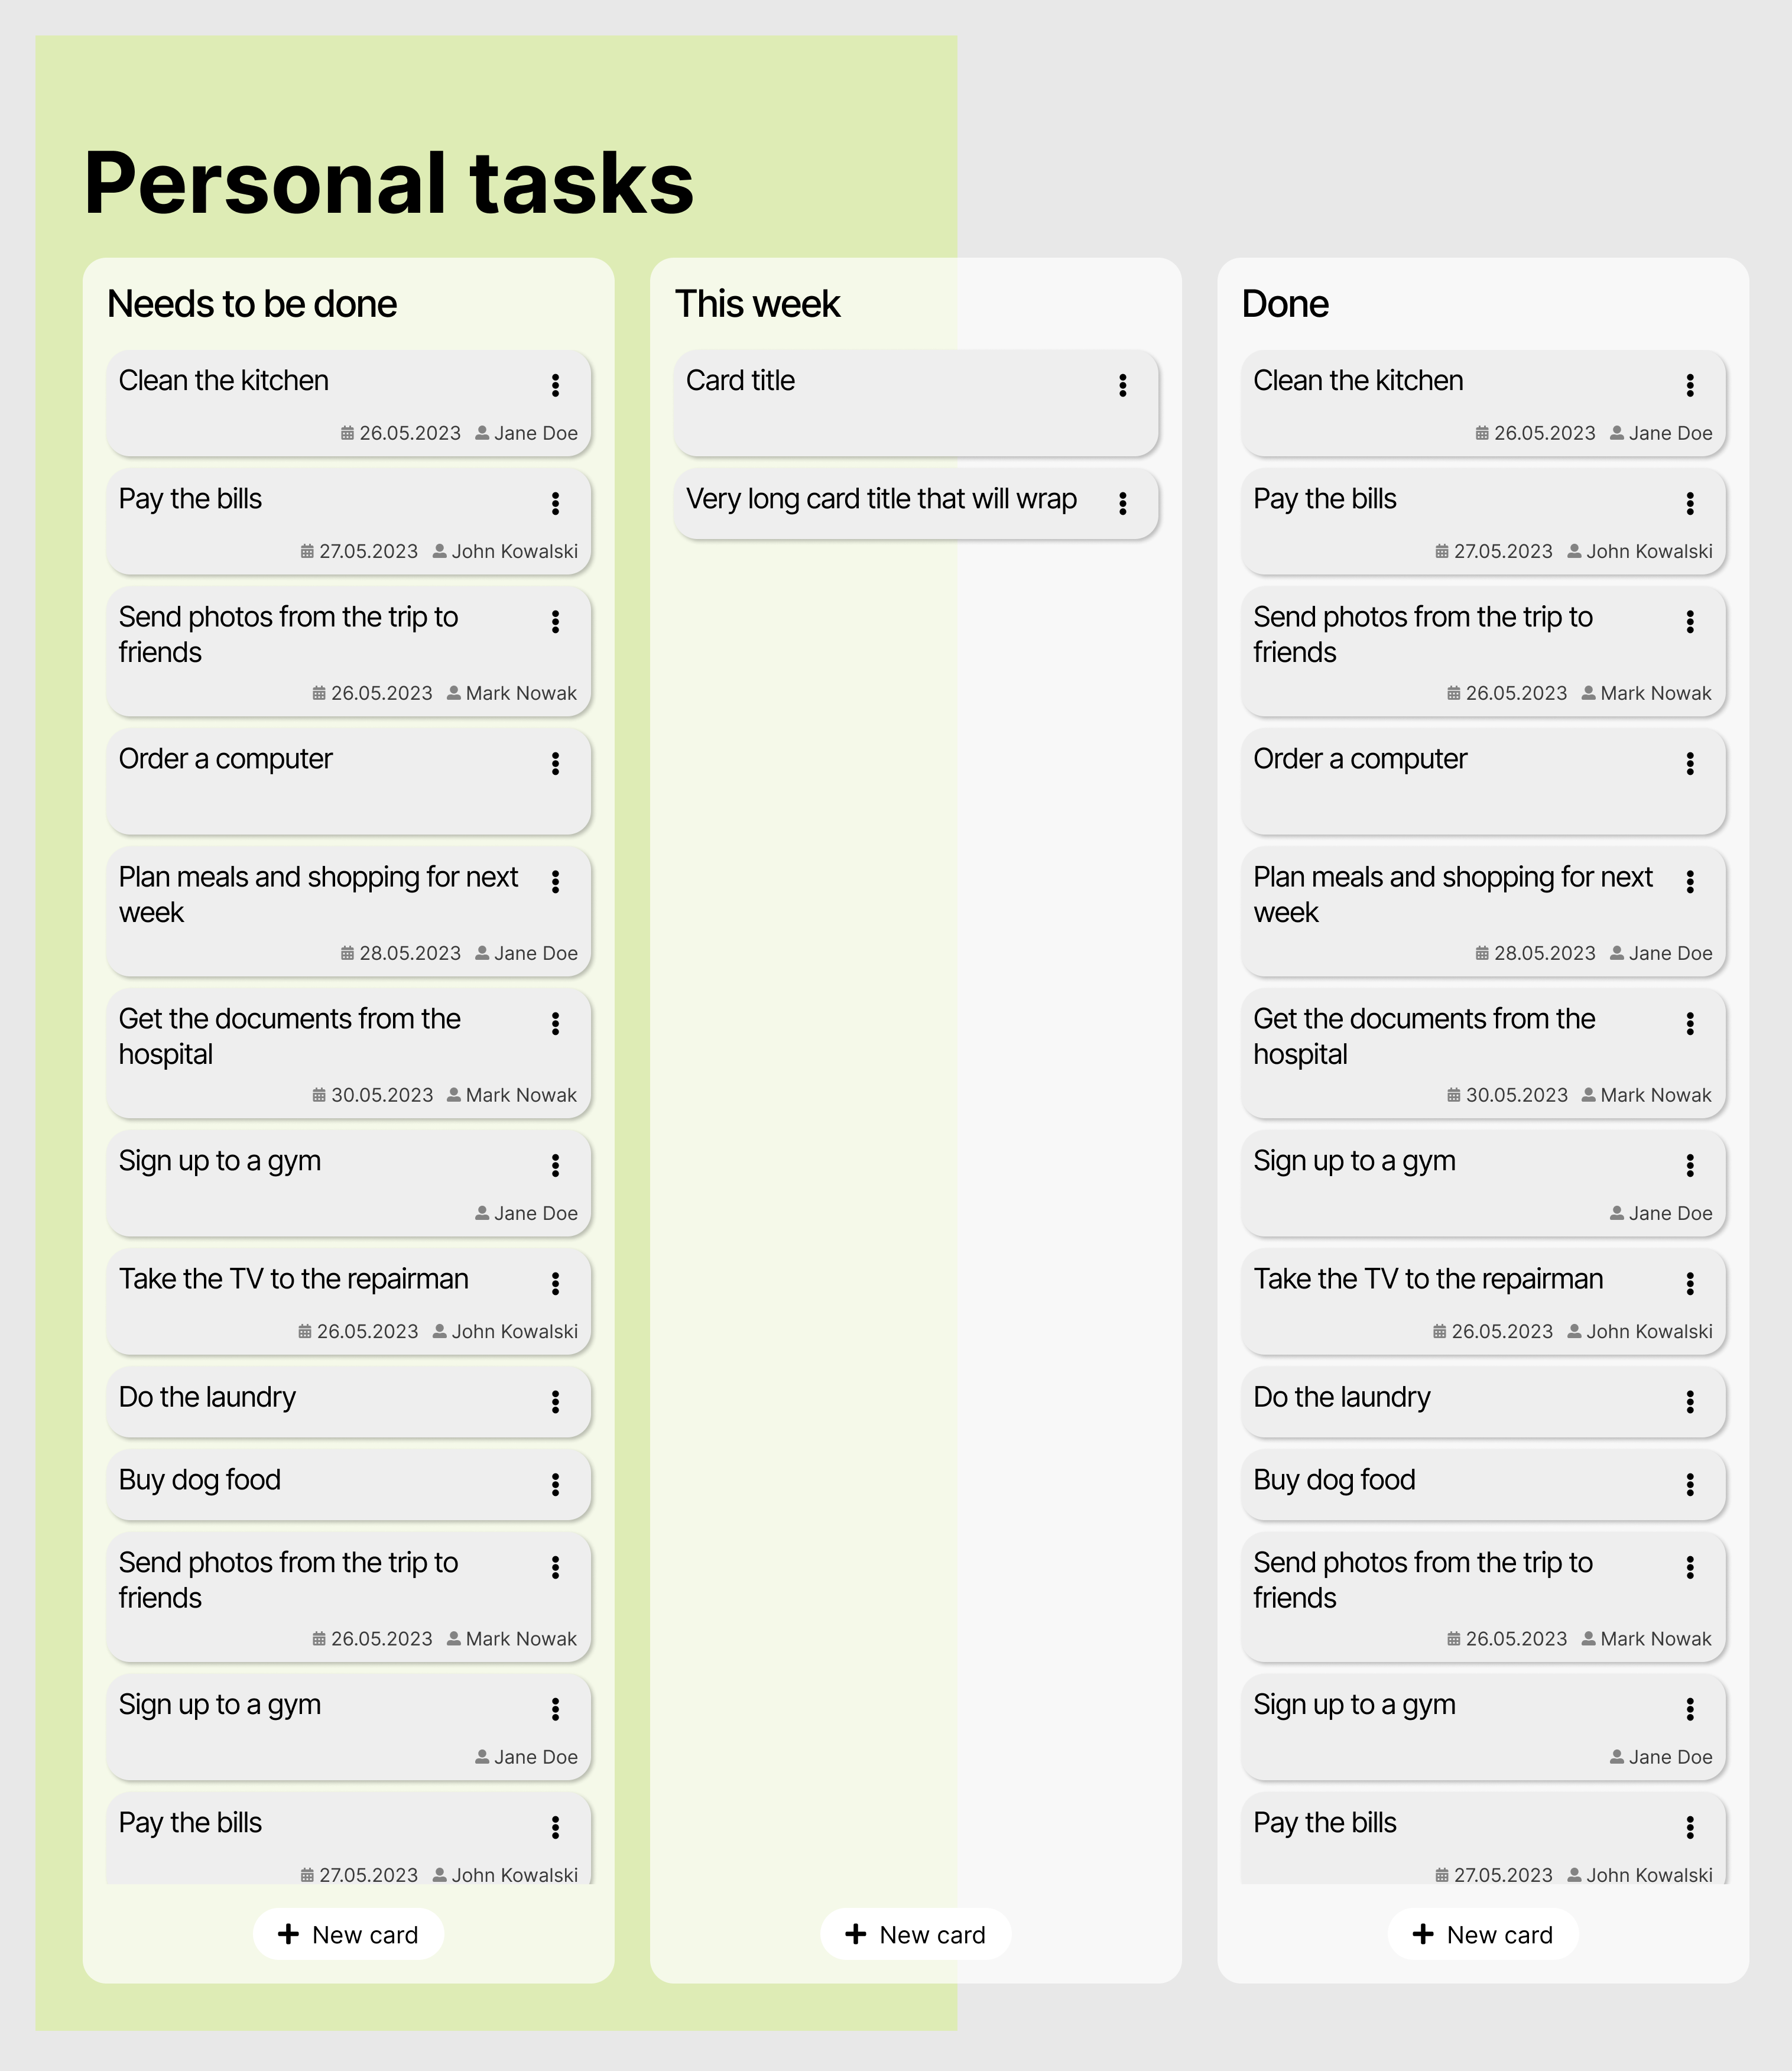
\includegraphics[height=0.4\textheight]{./3-research-methodology/board-view}
    \caption{An example design of a board view.}
    \label{fig:3-4-board-view}
\end{figure}

\begin{figure}
    \centering
    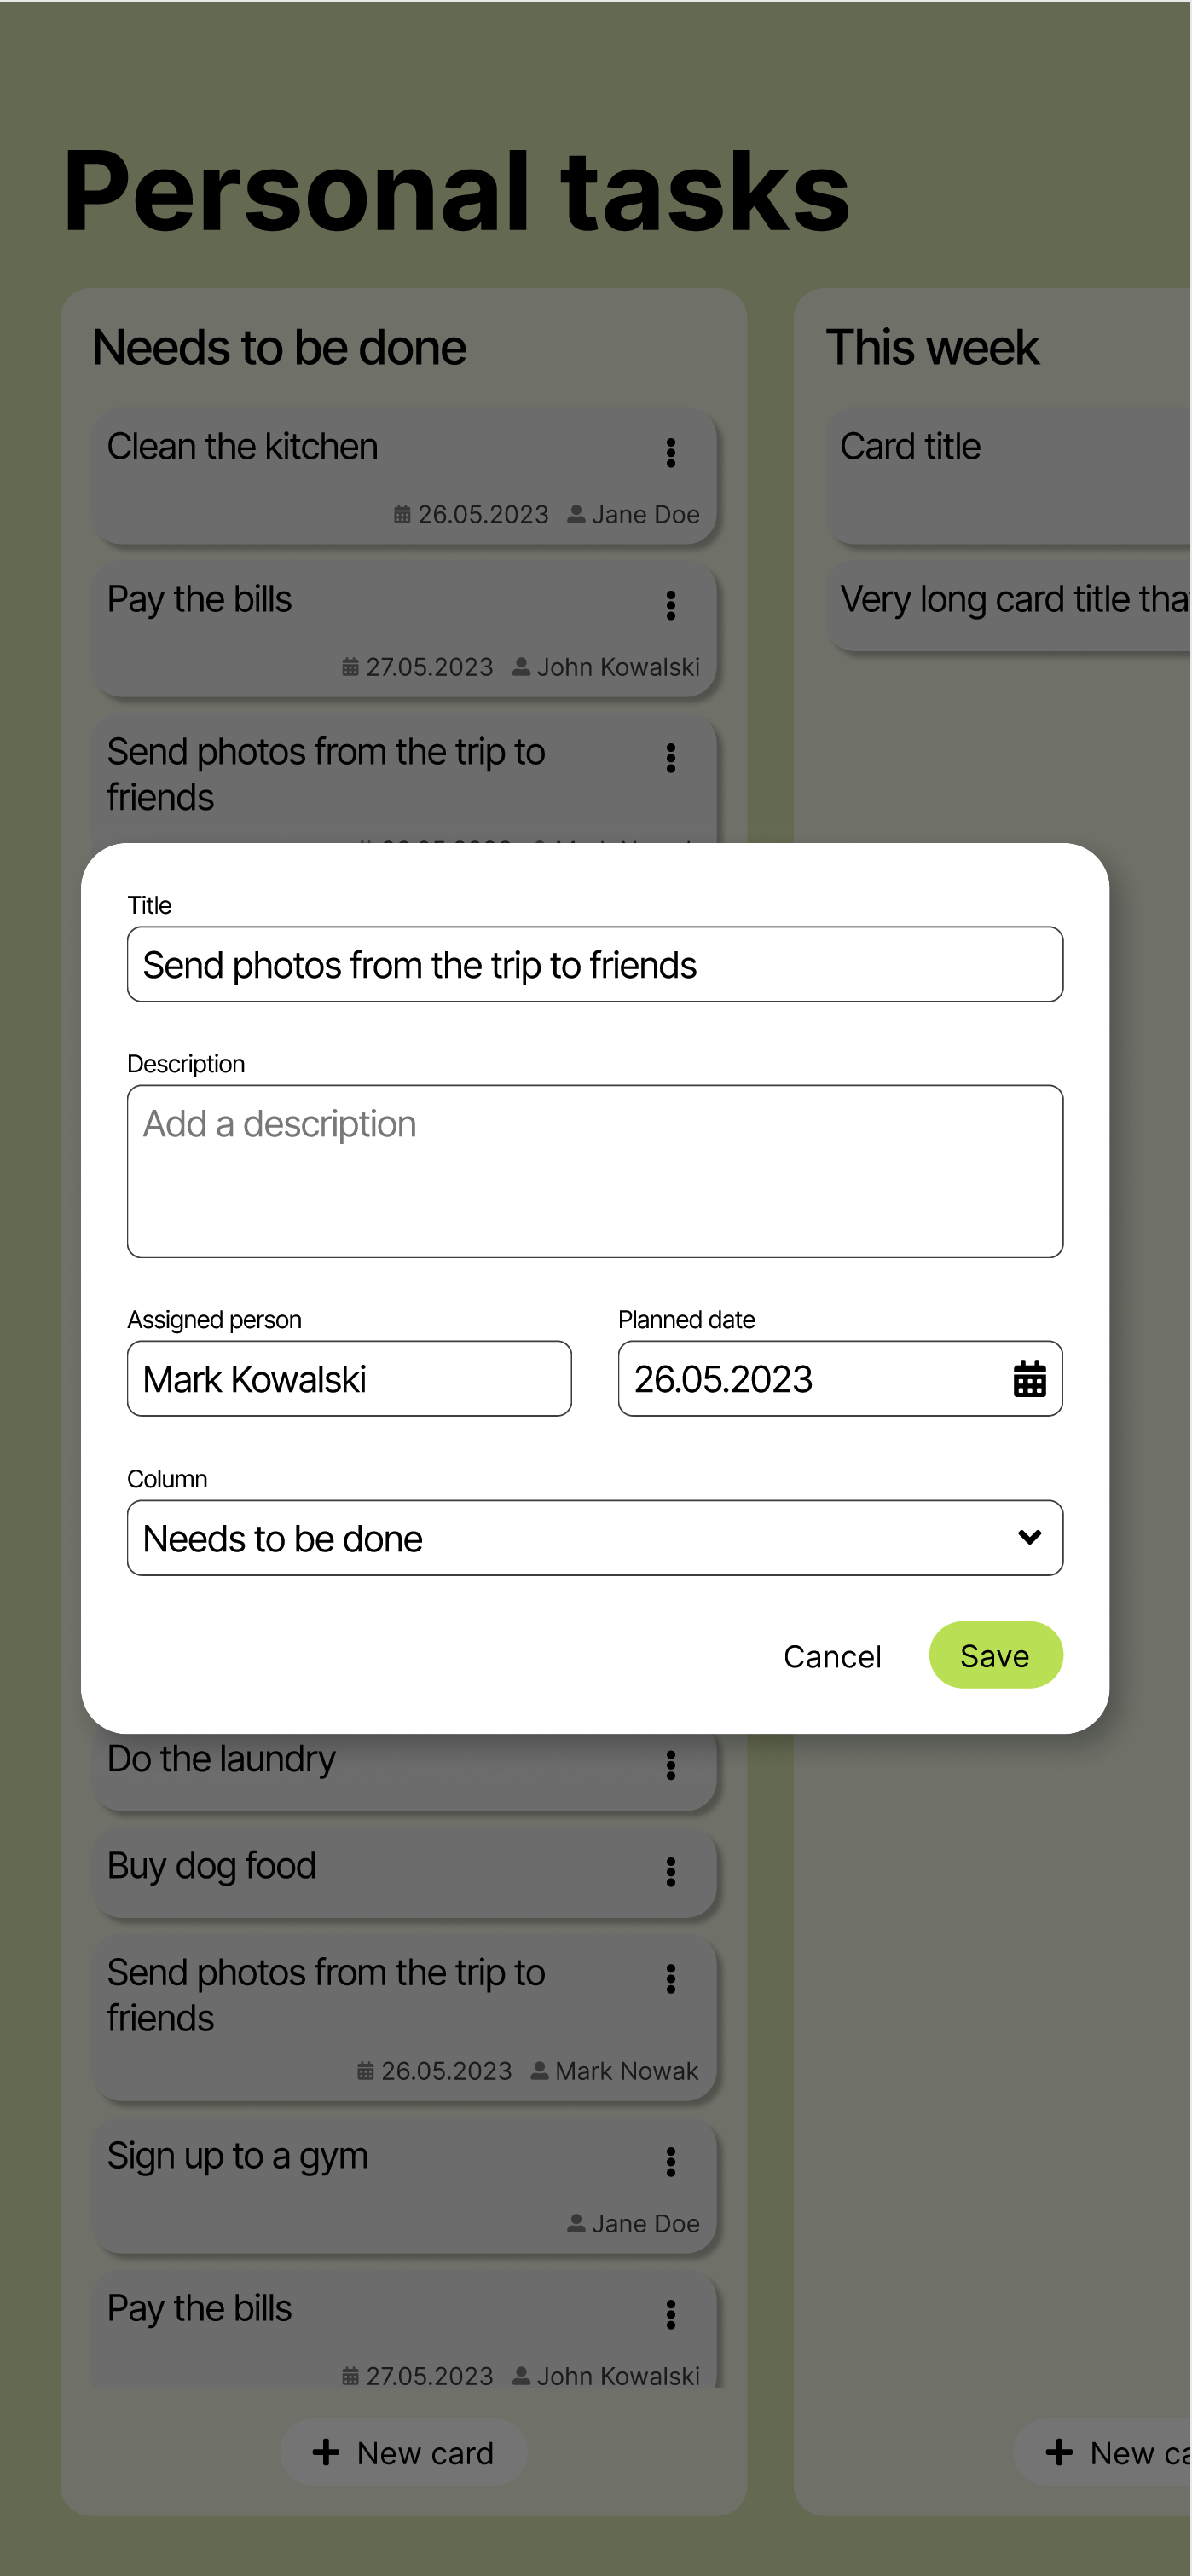
\includegraphics[height=0.4\textheight]{./3-research-methodology/board-view-with-dialog}
    \caption{An example design of a board view with the card editing dialog.}
    \label{fig:3-4-board-view-with-dialog}
\end{figure}

\todo[inline]{requirements}

\paragraph{The column component}
The column component, presented in figure~\ref{fig:3-4-column-component} consists of three parts: a title at the top, a set of cards and a button for adding new cards in the bottom.
The button opens a dialog window with a form for providing data about the card.
The top and bottom parts are \enquote{stuck} to the edges of the container: the title is always on the top of the container and the button \textendash\ at the bottom;
cards take the rest of the space of the container, scrolling if they cannot fit.

\begin{figure}
    \centering
    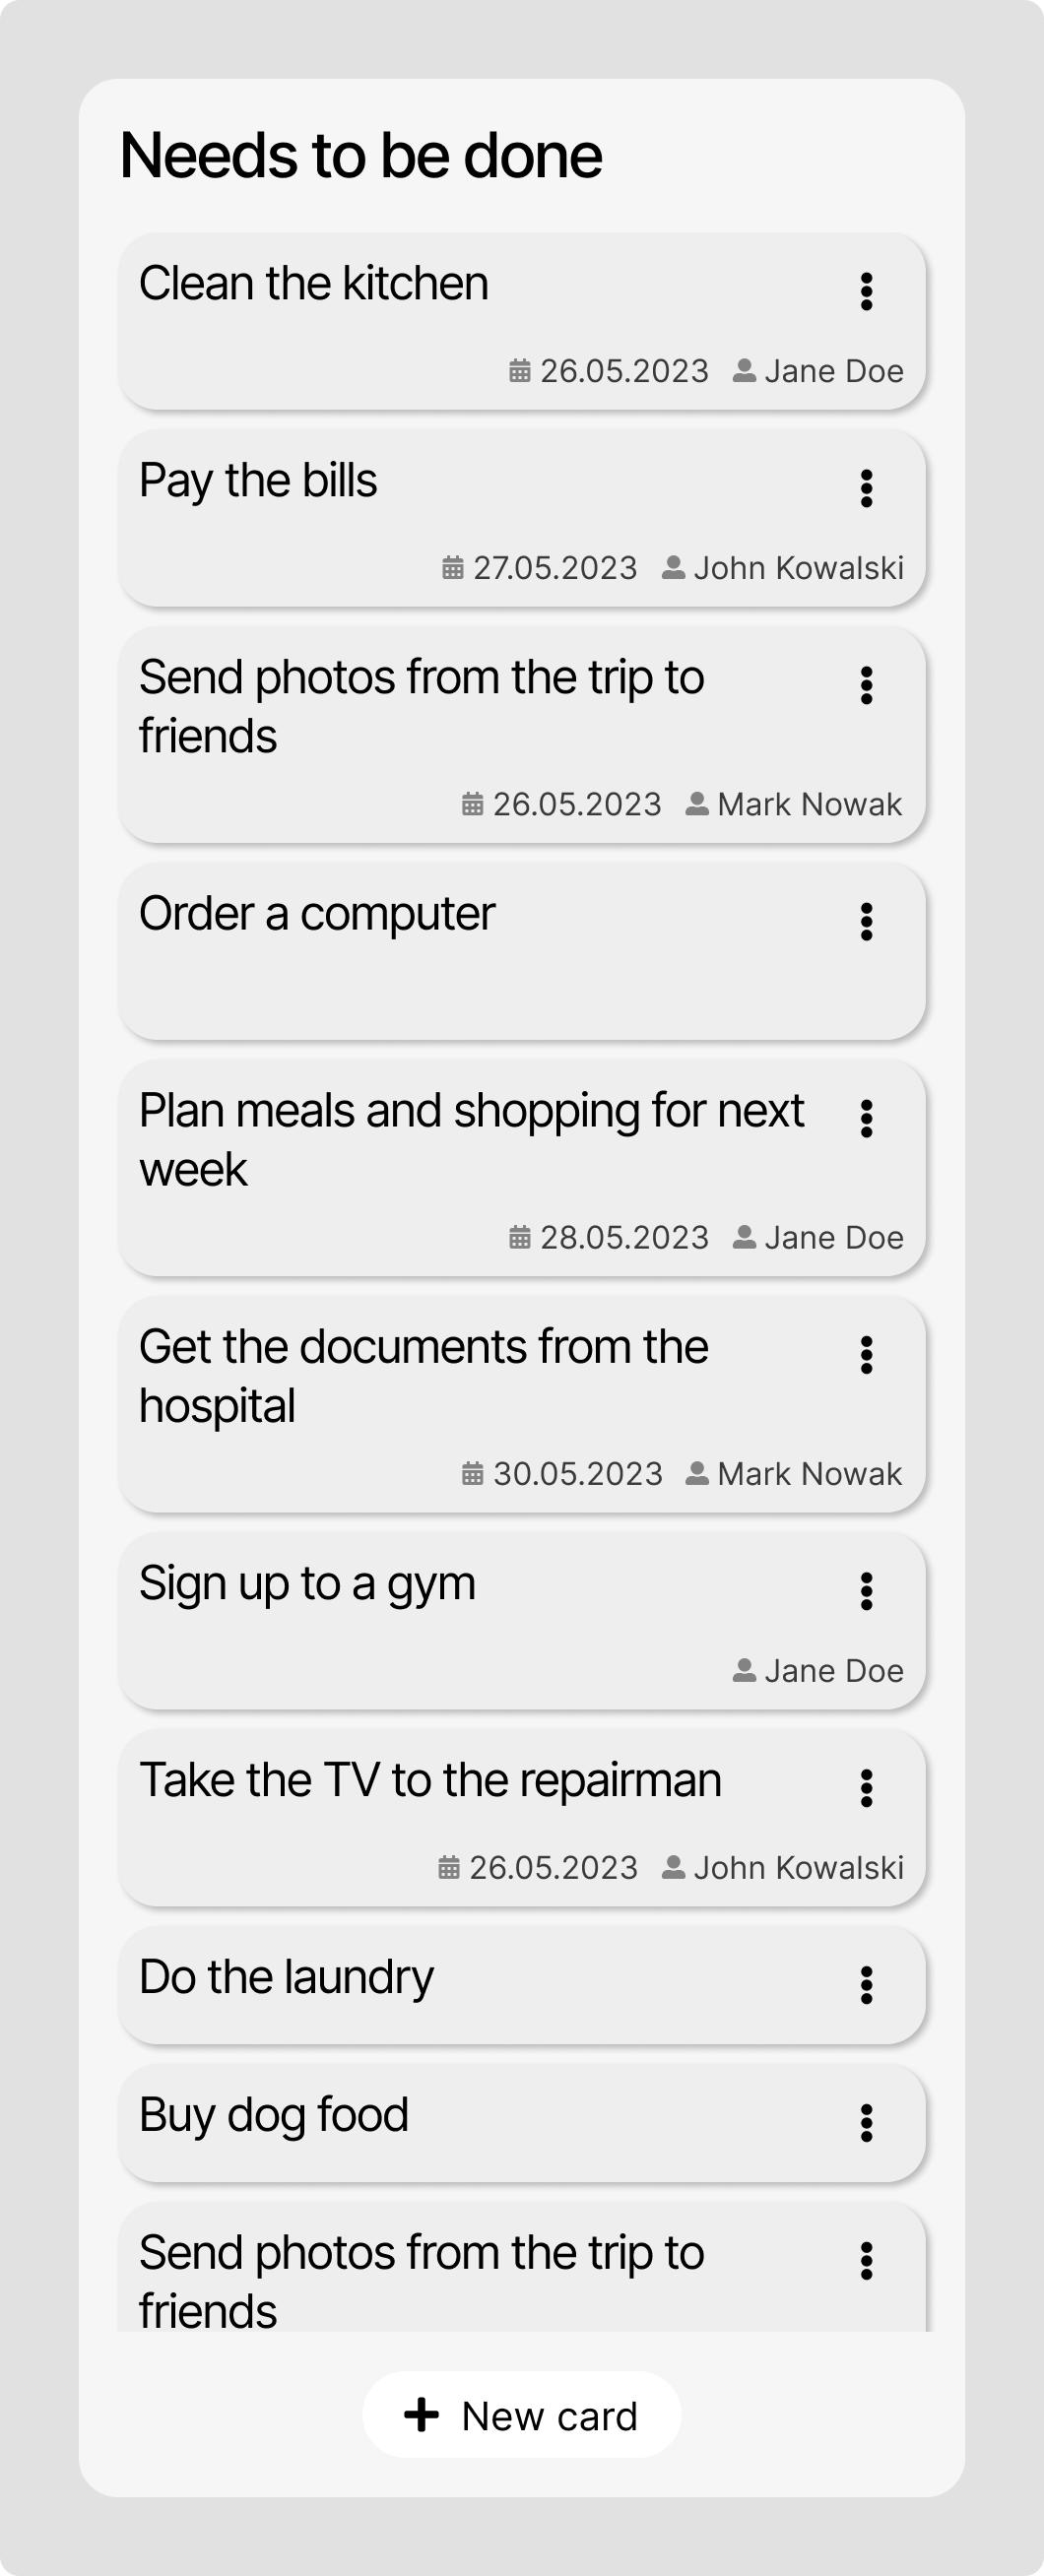
\includegraphics[height=0.5\textheight]{./3-research-methodology/column-component}
    \caption{An example design of a column component.}
    \label{fig:3-4-column-component}
\end{figure}

\todo[inline]{requirements}

\paragraph{The card component}
Figures~\ref{fig:3-4-card-component} and~\ref{fig:3-4-card-component-with-menu} depict a card component, consisting of a title and various indicators (short texts with an icon) \textendash\ that unobtrusively signal information about a list item.
In the top-right corner of the card there is a button that opens a context menu with two items: one that allows for editing a card (by opening a dialog), and the other that deletes a card.

\begin{figure}
    \centering
    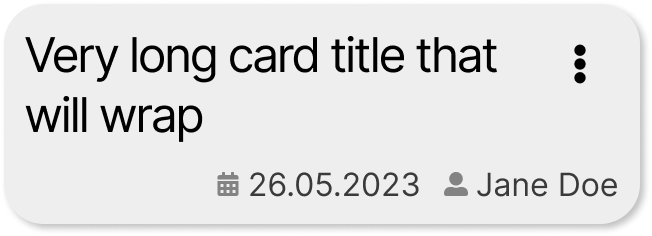
\includegraphics[width=\textwidth]{./3-research-methodology/card-component}
    \caption{An example design of a card component.}
    \label{fig:3-4-card-component}
\end{figure}

\begin{figure}
    \centering
    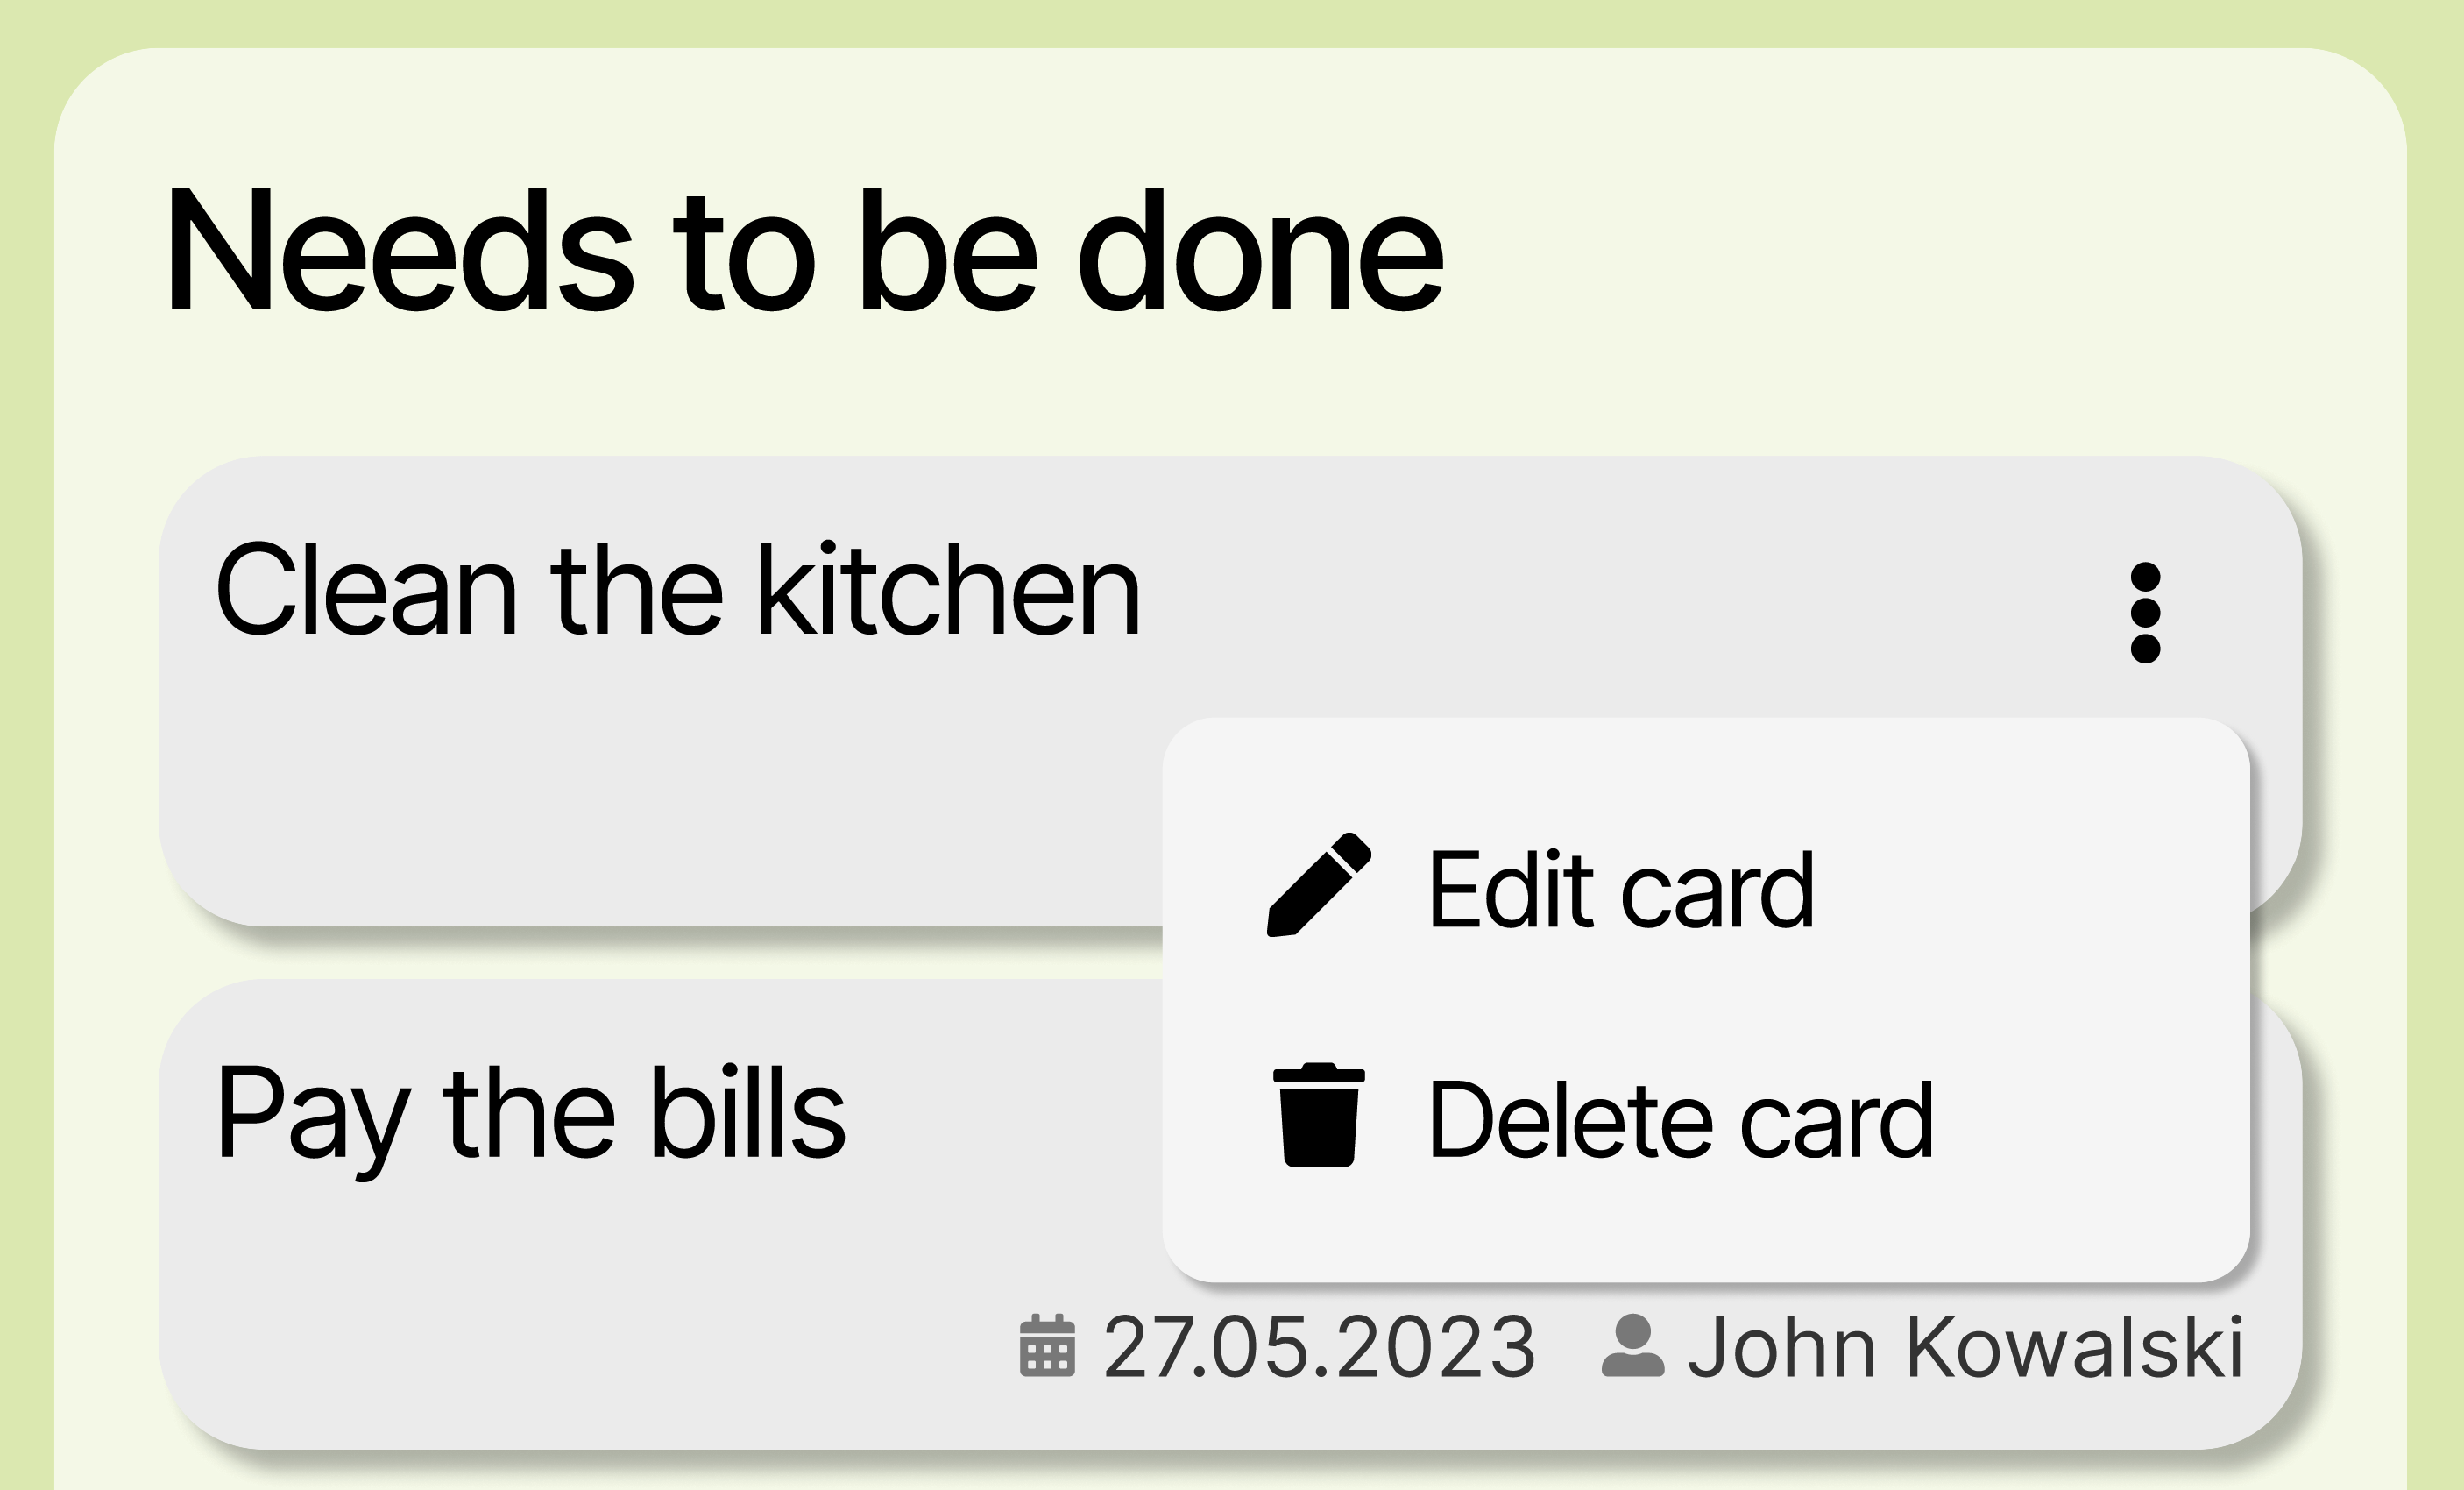
\includegraphics[width=\textwidth]{./3-research-methodology/card-component-with-menu}
    \caption{An example design of a card component with menu opened.}
    \label{fig:3-4-card-component-with-menu}
\end{figure}

\paragraph{The card editing dialog}
The dialog is presented in the figures~\ref{fig:3-4-card-dialog} and~\ref{fig:3-4-card-dialog-with-error}.
It is essentially a simple form \textendash\ a user can use it to provide information about a card: a title, a description, a person responsible for the card, a date and the column.
Two buttons are placed at the bottom of the view \textendash\ one for discarding the edits and the other one for saving them.
Only the title field is explicitly validated as a mandatory field.
\todo{write clearer}The column field is also required, but it should be chosen from a given set of values, therefore it does not need any additional validation.
The rest of the fields are optional.
\todo[inline]{requirements}

\begin{figure}
    \centering
    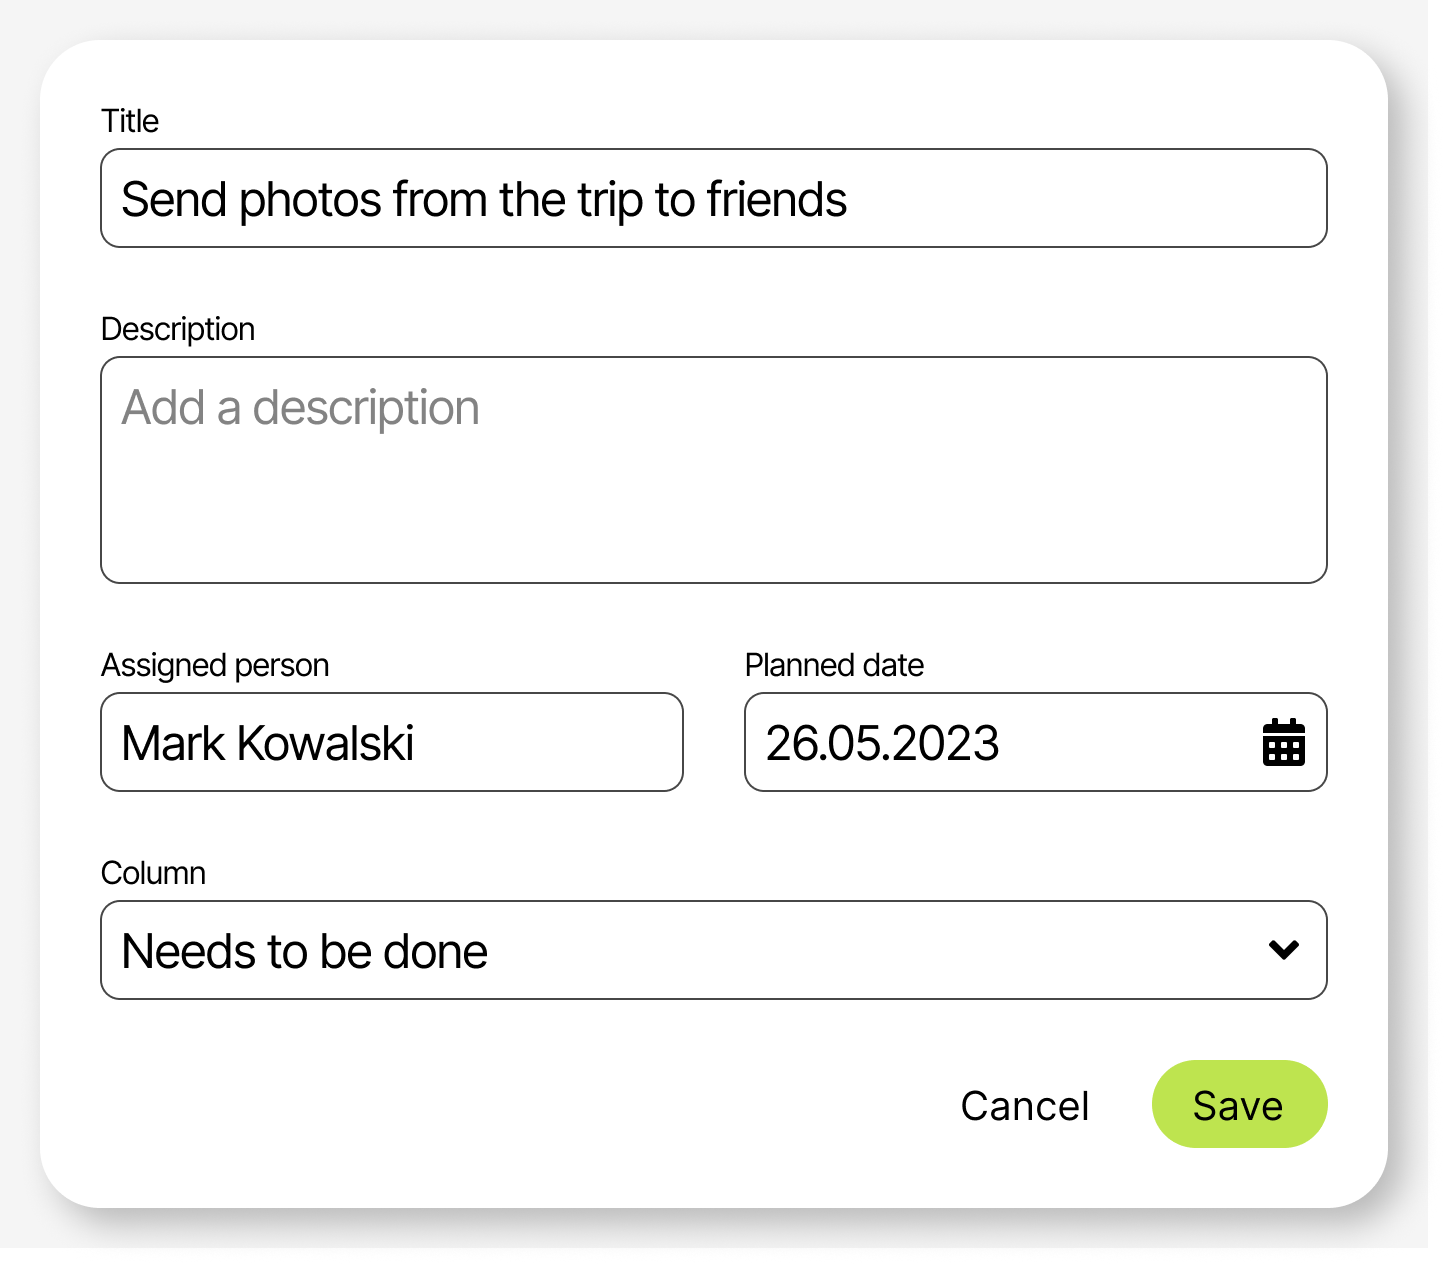
\includegraphics[height=0.4\textheight]{./3-research-methodology/card-dialog}
    \caption{An example design of a card editing dialog.}
    \label{fig:3-4-card-dialog}
\end{figure}

\begin{figure}
    \centering
    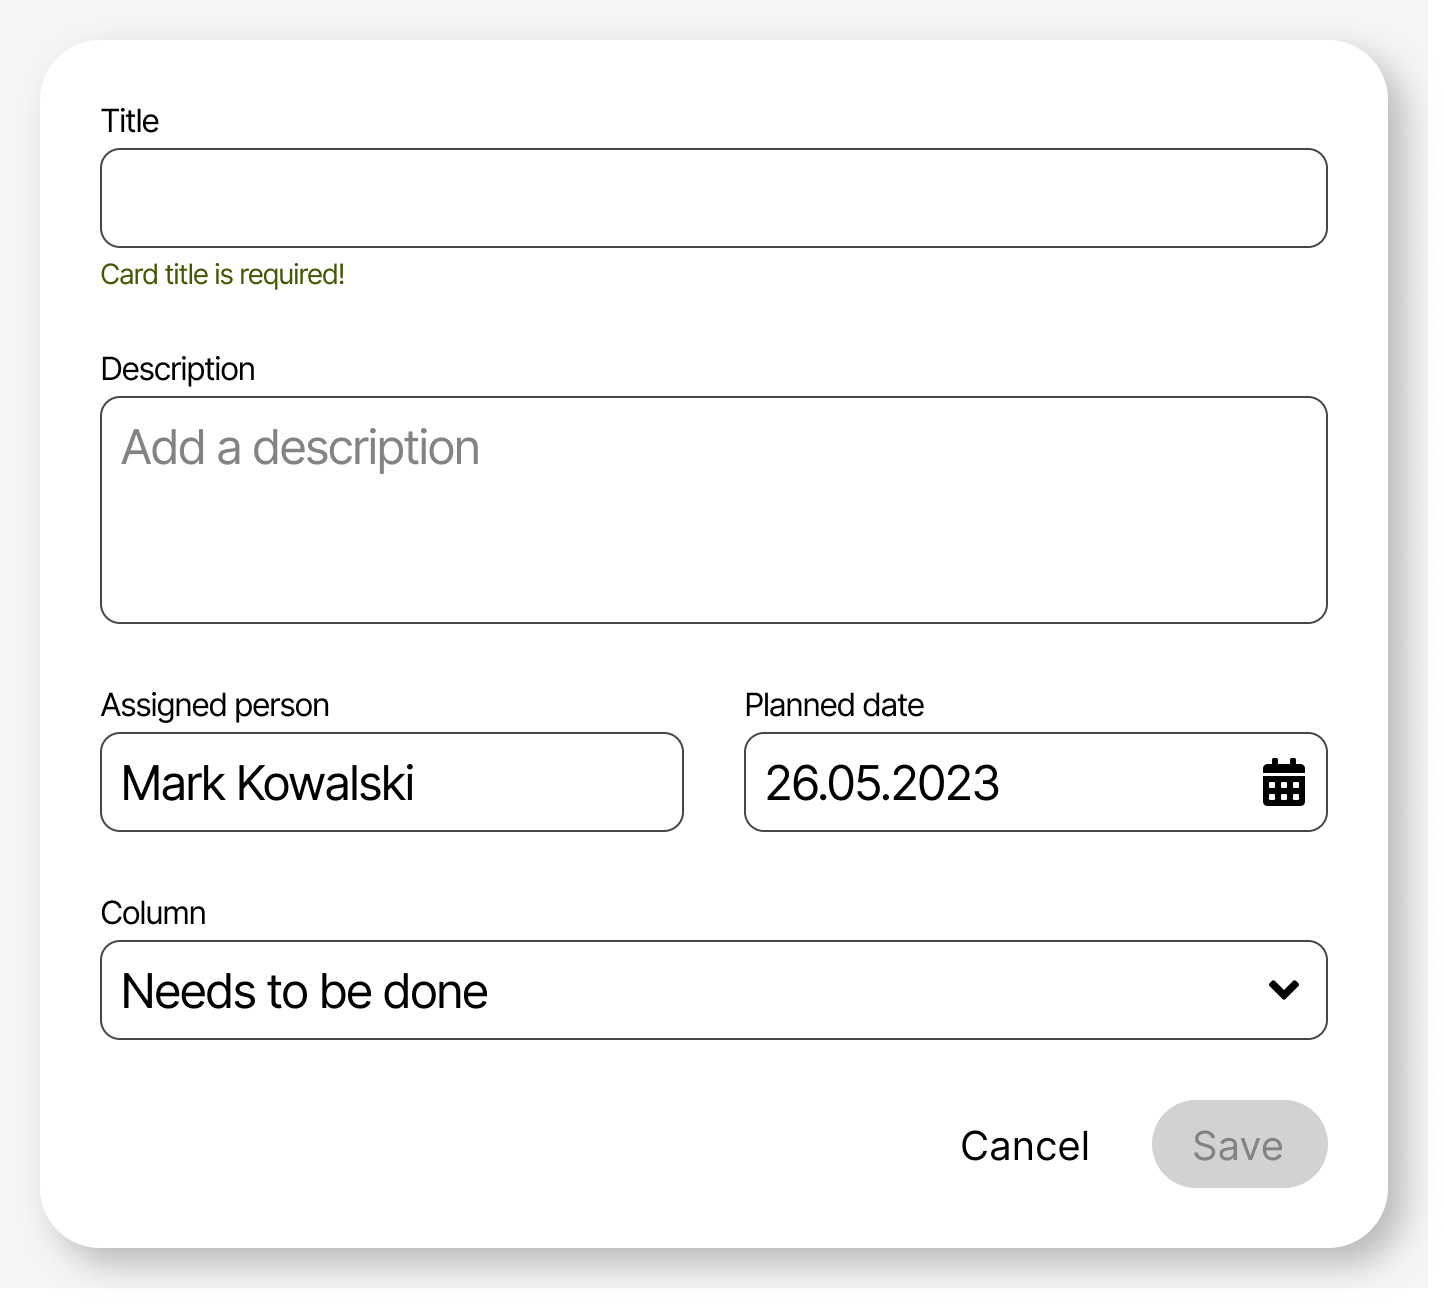
\includegraphics[height=0.4\textheight]{./3-research-methodology/card-dialog-with-error}
    \caption{An example design of a card editing dialog with input error.}
    \label{fig:3-4-card-dialog-with-error}
\end{figure}

